%\PassOptionsToPackage{svgnames}{xcolor}
\documentclass{article}
\usepackage{geometry}
\usepackage[utf8]{inputenc, vietnam}
\usepackage{tcolorbox}
\usepackage{amsmath, amssymb, amsthm}
\usepackage{pdfpages}

\definecolor{black}{rgb}{0.0, 0.0, 0.0}
\definecolor{blue}{rgb}{0.0, 0.0, 255.0}
\definecolor{green}{rgb}{0.0, 255.0, 0.0}
\definecolor{cyan}{rgb}{0.0, 255.0, 255.0}
\definecolor{red}{rgb}{255.0, 0.0, 0.0}
\definecolor{magenta}{rgb}{255.0, 0.0, 255.0}
\definecolor{yello}{rgb}{255.0, 255.0, 0.0}
\definecolor{white}{rgb}{255.0, 255.0, 255.0}

\geometry{a5paper}

\newcommand{\rank}{\text{rank}}

\theoremstyle{definition}
\newtheorem{definition}{Định nghĩa}[section]
\newtheorem*{remark}{Nhận xét}

\renewcommand*\contentsname{Mục lục}

\title{Nơi huyền thoại lưu danh}   
\author{Lê Quốc Dũng} 
\date{\today} 

\begin{document}

\newenvironment{myexampleblock}[1]{%
    \tcolorbox[colback=LightGreen,colframe=DarkGreen,title=#1]}
    {\endtcolorbox}

\newenvironment{defblock}[2]{%
    \tcolorbox[colback=white,colframe=blue,title=#1
    ]}
    {\endtcolorbox}

\newenvironment{theoremblock}[2]{%
    \tcolorbox[colback=white,colframe=magenta,title=#1
    ]}
    {\endtcolorbox}

%=========================================
\begin{titlepage}
		\centering{
			{\fontsize{40}{48}\selectfont 
			Nơi huyền thoại lưu danh}
		}\\
			
		\vspace{10mm}
		\centering{\Large{Lê Quốc Dũng}}\\
		\vspace{\fill}
		\centering \large{2023}
\end{titlepage}

\newpage
%\thispagestyle {empty}

\vspace*{2cm}

\begin{center}
	\Large{\parbox{10cm}{
		\begin{raggedright}
		{\Large 
			\textit{Đường đi ngàn dặm, bắt đầu bằng một bước chân.}
		}
	
		\vspace{.5cm}\hfill{Lão Tử}
		\end{raggedright}
	}
}
\end{center}

\newpage

\tableofcontents

\newpage

\textbf{Bảng các ký hiệu dùng trong sách}

\begin{table}[h]
    \begin{tabular}{c c}
        $\# S$ & số lượng phần tử của tập hợp $S$ (lực lượng của $S$)
    \end{tabular}
\end{table}

\newpage

\section{Đại số tuyến tính}

\subsection{Nhắc lại các khái niệm cơ bản}

\begin{defblock}{Hạng của ma trận}
    
    Cho ma trận $\mathbf{M}_{m \times n}$ có $m$ hàng và $n$ cột. \textbf{Hạng} của ma trận $\mathbf{M}$ là cấp của ma trận vuông con lớn nhất của $\mathbf{M}$ có định thức khác 0.

    \textit{Ký hiệu}. Hạng (hay rank) của ma trận $\mathbf{M}$ ký hiệu là $r = \rank(\mathbf{M})$

    \textit{Nhận xét}. Nếu $r$ là hạng của ma trận $\mathbf{M}_{m \times n}$ thì $r \leq \min (m, n)$
\end{defblock}

\newpage

\chapter{Mở đầu về số học}

Số học xuất hiện từ xa xưa, từ những bước đi đầu tiên của con
người. Tuy nhiên số học lại mang vẻ bí ẩn khó tưởng, sự phức
tạp vượt ra phạm vi số học. Nhà toán học vĩ đại Gauss từng nói
\textit{Toán học là vua của các môn khoa học, và số học là
nữ hoàng}. Hay một trong 23 bài toán thế kỷ của Hilbert về sự
phi mâu thuẫn của số học, người ta đã chứng minh được rằng
không thể chứng minh sự phi mâu thuẫn của số học chỉ bằng các
lý thuyết về số học.

\section{Phép chia Euclid}

Đây là nền tảng, cơ sở của số học. Từ khi biết tới phép chia
hai số nguyên, ta có thể tìm \textit{thương} và \textit{số dư}.
Nói theo toán học, nếu ta có 2 số nguyên dương $a$ và $b$, thì
tồn tại cặp số $q$, $r$ sao cho $a = qb + r$ với $0 \leq r < b$.

Khi đó, $a$ gọi là số bị chia, $b$ gọi là số chia, $q$ là thương
(q trong quotient) và $r$ là số dư (r trong remainder).

Đặc biệt là sự tồn tại của cặp số $q$ và $r$ là duy nhất. Thật
vậy, nếu ta giả sử tồn tại 2 cặp số $(q_1, r_1)$ và $(q_2, r_2)$ 
đều thỏa đẳng thức trên, nghĩa là
\[a = q_1 b + r_1, \quad a = q_2 b + r_2\]

Trừ 2 đẳng thức vế theo vế ta có $(q_1 - q_2) b + (r_1 - r_2) = 0$.
Tương đương $(r_2 - r_1) = (q_1 - q_2) b$, mà $0 \leq r_1, r_2 < b$
nên $-b < r_2 - r_1 < b$. Như vậy chỉ có thể xảy ra trường hợp
$r_2 - r_1 = 0$ hay $r_2 = r_1$, kéo theo $q_1 = q_2$.

\section{Thuật toán Euclid}

Dựa trên phép chia Euclid, ta có một thuật toán hiệu quả để tìm
ước chung lớn nhất giữa hai số $a$ và $b$.

Ký hiệu $\gcd(a, b)$ là ước chung lớn nhất của $a$ và $b$. Chúng 
ta thực hiện đệ quy như sau:
\[\gcd(a, b) = \begin{cases}
    a, \quad & \text{nếu}\,b = 0 \\
    \gcd(b, a \bmod b), \quad & \text{nếu}\,b \neq 0
\end{cases} 
    \]

Điểm quan trọng ở thuật toán Euclid là thuật toán chắc chắn sẽ dừng
sau một số hữu hạn bước, và kết quả sẽ là ước chung lớn nhất của 2
số $a$ và $b$.

\chapter{Lý thuyết nhóm}

Câu chuyện bắt đầu vào một ngày khi mình vẫn còn sống ngày tháng tươi đẹp.

Cho tới khi học \textbf{lý thuyết nhóm} thì đời bớt đẹp hơn tí.

Để bắt đầu mình cần hiểu nhóm là gì.

\section{Nhóm}

%\begin{defblock}{Nhóm (Group)}
\begin{definition}{Nhóm (Group)}
    Một tập hợp $G$ và toán tử 2 ngôi $\star$ trên $G$ tạo thành một nhóm nếu:
    \begin{enumerate}[noitemsep]
        \item Tồn tại phần tử $e \in G$ sao cho với mọi $g \in G$ thì $g \star e = e \star g = g$. Khi đó $e$ được gọi là \textbf{phần tử đơn vị} của $G$.
        \item Với mọi $g \in G$, tồn tại $g' \in G$ sao cho $g \star g' = g' \star g = e$. Khi đó $g'$ được gọi là \textbf{phần tử nghịch đảo} của $g$.
        \item Tính kết hợp: với mọi $a, b, c \in G$ thì $a \star (b \star c) = (a \star b) \star c$.
    \end{enumerate}
\end{definition}

%\end{defblock}

%\begin{defblock}{Nhóm Abel}
\begin{definition}{Nhóm Abel}
    Nếu nhóm $G$ có thêm tính giao hoán, tức là với mọi $a, b \in G$ thì $a \star b = b \star a$ thì $G$ gọi là nhóm giao hoán hay nhóm Abel
\end{definition}
%\end{defblock}

Lý thuyết nhóm thuộc toán trừu tượng, và nó trừu tượng thật. Tuy nhiên khi học về nó mình dần hiểu hơn về cách toán học vận hành và phát triển.

\begin{example}
    Xét tập hợp số nguyên $\ZZ$ và phép cộng 2 số nguyên.
    \begin{enumerate}[noitemsep]
        \item Phần tử đơn vị là 0 vì với mọi $a \in \ZZ$ thì $a + 0 = 0 + a = a$
        \item Với mọi $a \in \ZZ$, phần tử nghịch đảo là $-a$ vì $a + (-a) = (-a) + a = 0$
        \item Phép cộng số nguyên có tính kết hợp do đó thỏa mãn điều kiện về tính kết hợp
    \end{enumerate}
    Như vậy $(\ZZ, +)$ tạo thành nhóm. Lưu ý do phép cộng 2 số nguyên có tính giao hoán nên đây cũng là nhóm Abel.
\end{example}

\begin{example}
    Xét tập hợp số hữu tỉ khác 0 $\QQ^*$ và phép nhân 2 số hữu tỉ. Ta thấy do $a, b \in \QQ^*$ nên tích $a \cdot b$ cũng khác 0, do đó cũng thuộc $\QQ^*$.
    \begin{enumerate}[noitemsep]
        \item Phần tử đơn vị là 1 vì với mọi $a \in \QQ^*$ thì $a \cdot 1 = 1 \cdot a = a$
        \item Với mọi $a \in \QQ^*$, phần tử nghịch đảo là $\frac{1}{a}$ vì $a \cdot \frac{1}{a} = \frac{1}{a} \cdot a = 1$
        \item Phép nhân 2 số hữu tỉ có tính giao hoán do đó thỏa mãn điều kiện về tính kết hợp
    \end{enumerate}
    Tương tự như nhóm $\mathbb{Z, +}$, nhóm $(\QQ^*, \cdot)$ cũng là nhóm Abel.
\end{example}

\section{Nhóm con}

\begin{definition}{Nhóm con (Subgroup)}
    Cho nhóm $(G, \star)$. Tập hợp $H \subset G$ được gọi là \textit{nhóm con} của $G$ nếu với mọi $a, b \in H$ thì $a \star b \in H$
\end{definition}
 
Nghĩa là toán tử $\star$ đóng với các phần tử trong $H$.

\begin{example}
    Xét nhóm $(\ZZ, +)$ như trên. Ta xét tập con gồm các số chẵn của nó
    \[2\ZZ = \{\ldots, -4, -2, 0, 2, 4, \ldots\}\]

    Ta thấy rằng tổng 2 số chẵn vẫn là số chẵn, nghĩa là phép cộng số nguyên đóng trên $2\ZZ$.
    Do đó $(2\ZZ, +)$ là nhóm con của $(\ZZ, +)$.

    Như vậy mọi tập hợp có dạng $n \ZZ$ đều là nhóm con của $(\ZZ, +)$.
\end{example}

\section{Coset}

\begin{definition}{Coset}
    (tạm dịch - \textit{lớp kề} theo wikipedia) Cho nhóm $G$ và nhóm con $H$ của $G$.

    Coset trái của $H$ đối với phần tử $g \in G$ là tập hợp
    \[gH = \{gh : h \in H \}\]

    Tương tự, coset phải là tập hợp
    \[Hg = \{hg : h \in H \}\]
\end{definition}

Từ đây nếu không nói gì thêm ta ngầm hiểu là coset trái.

Ví dụ với nhóm con $2\ZZ$ của $\ZZ$, ta thấy rằng

\begin{enumerate}
    \item Nếu $g \in \ZZ$ là lẻ thì khi cộng với bất kì phần tử nào của $2\ZZ$ ta có số lẻ
    \item Nếu $g \in \ZZ$ là chẵn thì khi cộng với bất kì phần tử nào của $2\ZZ$ ta có số chẵn
\end{enumerate}

Nói cách khác, coset của $2\ZZ$ chia tập $\ZZ$ thành
\[0 (2\ZZ) = \{\ldots, -4, -2, 0, 2, 4, \ldots\}\]
 
\[1 (2\ZZ) = \{\ldots, -3, -1, 1, 3, \ldots \}\]

Trực quan mà nói, 2 coset trên rời nhau.

\begin{remark}
    Hai coset bất kì hoặc rời nhau, hoặc trùng nhau.
\end{remark}

\begin{proof}
    Nếu hai coset rời nhau thì không có gì phải nói. Ta chứng minh trường hợp còn lại.

    Giả sử $g_1 H \cap g_2 H \neq \emptyset$. Như vậy tồn tại $h_1, h_2 \in H$ mà $g_1 h_1 = g_2 h_2$.

    Do $h_1^{-1} \in H$, ta có $g_1 = g_2 h_2 h_1^{-1}$, nghĩa là $g_1 \in g_2 H$.

    Mà mọi phần tử trong $g_1 H$ có dạng $g_1 h$ nên $g_1 h = g_2 h_2 h_1^{-1} h$. Do $H$ là nhóm con của $G$ nên $h_2 h_1^{-1} h \in H$.
    Từ đó $g_1 H \subseteq g_2 H$. Tương tự ta cũng có $g_2 H \subseteq g_1 H$. Vậy $g_1 H = g_2 H$.
\end{proof}

\section{Normal Subgroup}

\begin{definition}{Normal Subgroup}
    (tạm dịch - \textit{nhóm con chuẩn tắc}) Nhóm con $H$ của $G$ được gọi là \textit{normal subgroup} nếu với mọi $g \in G$ ta có coset trái trùng với coset phải.
    \[gH = Hg \; \forall g \in G\]
\end{definition}

Nếu $H$ là normal subgroup của $G$ ta ký hiệu $H \triangleleft G$.

\begin{definition}{Quotient Group}
    (tạm dịch - \textit{nhóm thương}, hay Factor Group - \textit{nhóm nhân tử}). Với nhóm $G$ và normal subgroup của nó là $H$.
    Quotient Group được ký hiệu là $G / H$ và được định nghĩa là tập hợp các coset tương ứng với normal subgroup $H$.
    \[G / H = \{gH : g \in H \}\]

    Ta thấy rằng điều này chỉ xảy ra nếu $H$ là normal subgroup.
\end{definition}

\begin{example}
    Với nhóm $\ZZ$ và normal subgroup của nó là $2\ZZ$.
    Ta thấy $\ZZ / 2 \ZZ = \{0 + 2 \ZZ, 1 + 2 \ZZ\}$
\end{example}
\newpage

\section{Ba đường Conic}

Ba đường Conic bao gồm ellipse, hyperbol và parabol.

\subsection{Ellipse}

\begin{defblock}{Ellipse}

    Đường ellipse là tập hợp các điểm sao cho tổng khoảng cách từ nó tới 2 điểm cố định là 1 hằng số.
\end{defblock}

Nghĩa là, với 2 điểm cố định $F_1, F_2$, tập hợp các điểm $M$ sao cho $M F_1 + M F_2 = 2a$ với $a$ là hằng số tạo thành đường ellipse.

Ở trên hệ tọa độ, nếu ta chọn $F_1$ và $F_2$ nằm trên $Ox$ và đối xứng qua $Oy$, tức là $F_1 = (-c, 0)$ và $F_2 = (c, 0)$, thì các điểm $M = (x, y)$ nằm trên ellipse thỏa

$$MF_1 + MF_2 = \sqrt{(x+c)^2 + y^2} + \sqrt{(x-c)^2 + y^2} = 2a$$

Tương ứng với biển đổi thành phương trình

$$\frac{x^2}{a^2} + \frac{y^2}{a^2 - c^2} = 1$$

Đặt $b^2 = a^2 - c^2$ thì phương trình của ellipse trở thành

$$\frac{x^2}{a^2} + \frac{y^2}{b^2} = 1$$

Phương trình này gọi là \textbf{phương trình chính tắc}.

\begin{figure}[ht]
    \centering
    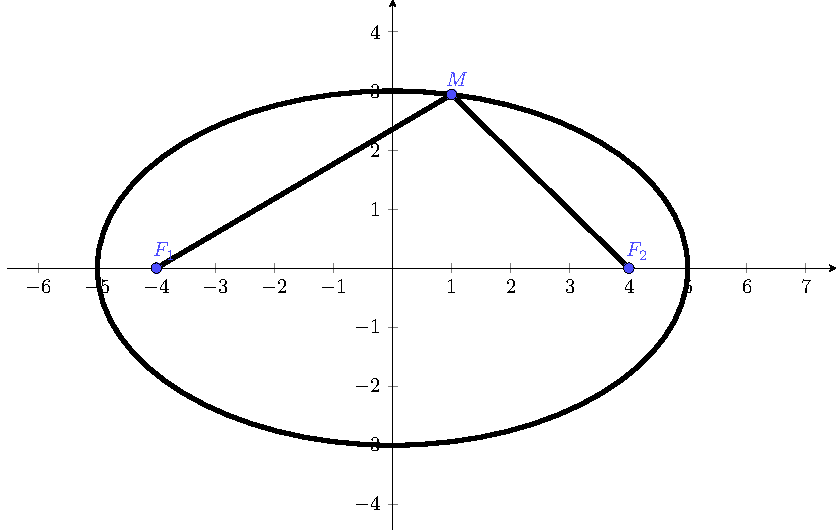
\includegraphics[width=\textwidth]{pics/conics/ellipse.pdf}
    \caption{Ellipse với phương trình $\frac{x^2}{25} + \frac{y^2}{9} = 1$}
\end{figure}

Trong phương trình $$\frac{x^2}{a^2} + \frac{y^2}{b^2} = 1$$

thì $a$ là khoảng cách từ tâm tới 2 biên trái hoặc phải, nên $a$ là \textbf{độ dài bán trục lớn}.

Tương tự, $b$ là \textbf{độ dài bán trục nhỏ} (khoảng cách từ tâm tới 2 biên trên dưới).

Từ cách đặt $b^2 = a^2 - c^2$ tương đương $c^2 = a^2 - b^2$ thì $c$ gọi là \textbf{tiêu cự} của ellipse.

Các điểm $F_1, F_2$ gọi là \textbf{tiêu điểm} của ellipse.

Với ví dụ trên $\frac{x^2}{25} + \frac{y^2}{9} = 1$ thì $a=5, b=3$. Suy ra $c=4$ (lưu ý là $a, b > 0$ và $c \geq 0$).

Các đỉnh nằm ở các tọa độ $(-a, 0), (a, 0), (0, b), (0, -b)$. Các tiêu điểm nằm ở $(-c, 0), (c, 0)$.

\begin{remark}
    Khi $c=0$, tức là 2 tiêu điểm trùng nhau, ta có đường tròn.
\end{remark}

Tâm sai của ellipse là $e = \frac{c}{a} < 1$

\subsection{Hyperbol}

\begin{defblock}{Hyperbol}

    Đường hyperbol là tập hợp các điểm sao cho giá trị tuyết đối hiệu số khoảng cách từ nó tới 2 điểm cố định là 1 hằng số.
\end{defblock}

Nghĩa là, với 2 điểm cố định $F_1, F_2$, tập hợp các điểm $M$ sao cho $| M F_1 - M F_2 | = 2a$ với $a$ là hằng số tạo thành đường hyperbol.

Ở trên hệ tọa độ, nếu ta chọn $F_1$ và $F_2$ nằm trên $Ox$ và đối xứng qua $Oy$, tức là $F_1 = (-c, 0)$ và $F_2 = (c, 0)$, thì các điểm $M = (x, y)$ nằm trên hyperbol thỏa

$$| MF_1 - MF_2 | = | \sqrt{(x+c)^2 + y^2} - \sqrt{(x-c)^2 + y^2} | = 2a$$

Tương ứng với biển đổi thành phương trình

$$\frac{x^2}{a^2} - \frac{y^2}{a^2 - c^2} = 1$$

Đặt $b^2 = a^2 - c^2$ thì phương trình của hyperbol trở thành

$$\frac{x^2}{a^2} - \frac{y^2}{b^2} = 1$$

Đường hyperbol cắt trục $Ox$ tại 2 điểm $A_1 = (-a, 0)$ và $A_2 = (a, 0)$.

Tiêu điểm của hyperbol ở $F_1 = (-c, 0)$ và $F_2 = (c, 0)$.

Đường hyperbol có 2 tiệm cận là đường thẳng $y = \frac{b}{a} x$ và $y = -\frac{b}{a} x$.

Tâm sai của hyperbol là $e = \frac{c}{a} > 1$.

\subsection{Parabol}

\begin{defblock}{Parabol}

    Đường parabol là tập hợp các điểm cách đều một điểm cố định và một đường thẳng cố định.

\end{defblock}

Nghĩa là, với 1 điểm cố định $F$ và đường thẳng cố định $(d)$, parabol là tập hợp các điểm $M$ sao cho $MF = d(M, d)$ với $d(M, d)$ là khoảng cách từ $M$ tới đường thẳng $(d)$.

Phép dời tọa độ cho phép ta dời một hình parabol có đỉnh ở bất kì điểm nào về gốc tọa độ.

Tức là, không mất tính tổng quát, ta chỉ cần xét các parabol dạng $y=ax^2$ là đủ.

Điểm cố định ở trên được gọi là \textbf{tiêu điểm}. Đường thẳng cố định ở trên gọi là \textbf{đường chuẩn}.

Parabol có tính đối xứng nên tiêu điểm nằm trên $Oy$. Đặt tọa độ của nó là $F = (0, f)$.

Đường chuẩn nằm ngang nên ta có parabol là các điểm $M = (x, y)$ sao cho

$MF = \sqrt{x^2 + (y-f)^2}$ và $d(M, d) = y+f$ 
(trường hợp $M$ trùng với đỉnh nên điều kiện của parabol xảy ra tương đương với $M$ cách đều tiêu điểm và đường chuẩn, nghĩa là đường chuẩn có dạng $y=-f$).

Do đó $\sqrt{x^2 + (y-f)^2} = y + f$. Bình phương và biến đổi ta thu gọn được
$$f = \frac{1}{4a}$$

Thường thì ta đặt $p = f$, khi đó phương trình parabol trở thành 
$$x^2 = 4py$$

Đây là dạng chính tắc của parabol với trục đối xứng dọc.

Tâm sai của hyperbol là $e = \frac{c}{a} = 1$.
\newpage

\end{document}